
\usepackage{fancyhdr}
\usepackage{lastpage}
\usepackage[utf8]{inputenc}

% Minted for syntax highliting
\usepackage{minted}
\usemintedstyle{tango}

% Headers/footers styling
\pagestyle{fancy}
\fancyhf{}
\renewcommand{\headrulewidth}{0pt}

% Footer
\lfoot{ID1019}
\cfoot{KTH}
\rfoot{\thepage \hspace{1pt} / \pageref{LastPage}}

%\newcommand{\defaultpagestyle}{\thispagestyle{plain}}
\newcommand{\defaultpagestyle}{\thispagestyle{fancy}}


\title[ID1019 Summary]{Summary}


\author{Johan Montelius}
\institute{KTH}
\date{\semester}

\begin{document}

\begin{frame}
\titlepage
\end{frame}

\begin{frame}{evaluation}

A sequence is evaluated given an {\em environment}, written $\sigma$ (sigma).

\pause\vspace{20pt}
The environment holds a set of variable substitutions:
$v/s \in \sigma$ where $v$ is a variable and $s$ is a structure.

\pause\vspace{20pt} 
An evaluation of a sequence $e$ given an environment
$\sigma$ is written $E\sigma(e)$. 

\pause\vspace{20pt}
We write:
\vspace{20pt}
$$E\sigma(e) \rightarrow s$$
\vspace{20pt}
where $s$ is a data structure.

\end{frame}

\begin{frame}[fragile]{represent data structures}

\begin{verbatim}
-type structure() :: atom() | [atom()].
\end{verbatim}
\pause\vspace{20pt}

Examples of data structures:
\pause\vspace{20pt}
\begin{itemize}
\item an atom: {\tt a}, {\tt b}, {\tt []} or {\tt gurka}
\item a cons cell: {\tt [a | []]}, {\tt [a | [ b | []]]}
\end{itemize}

\pause\vspace{20pt}
Is this a data structure: {\tt [X | []]} ?

\end{frame}

\begin{frame}[fragile]{an environment}

\pause\vspace{20pt}
What is a good representation of an environment?

\pause\vspace{20pt}
\verb+[{x, foo}, {y, bar}, {z, [gurka|[]]}}]+

\pause\vspace{20pt}
\verb+ -type environment() :: [{atom(), structure()}]. +

\end{frame}

\begin{frame}[fragile]{env}

\begin{verbatim}
-moduel(env).

new() -> [].

bind(Var, Str) ->
   [{Var, Str}].

union(S1, S1) ->
   S1 ++ S2.

\end{verbatim}
\pause
\begin{verbatim}
lookup(Var, Env) ->
    lists:keyfind(Var, 1, Env).
\end{verbatim}

\end{frame}

\begin{frame}[fragile]{represent terms}

\begin{verbatim} 
-type term() :: {atm, atom()} | 
                {var, atom()} | 
                {cons,term(), term()}.
\end{verbatim} 

\pause\vspace{20pt}

\begin{itemize}
\item an atom : {\tt \{atm, a\}}, {\tt  \{atm, []\}}
\item a variable : {\tt \{var, x\}}, {\tt \{var, y\}}
\item a cons cell : {\tt \{cons, \{atm, a\}, \{atm, []\}\}}
\end{itemize} 

\end{frame}

\begin{frame}[fragile]{expressions} 

Let's have a limited number of expressions:

\pause\vspace{20pt}
\verb+ -type expression() :: term() | ... +
\pause\vspace{20pt}

\begin{itemize}
\item a term : {\tt \{atm a\}}, {\tt \{cons \{atm, a\}, \{[]\}}
\item a case expression : {\em more on this later}
\end{itemize}

\pause\vspace{20pt}
{\em No function application? }

\end{frame}

\begin{frame}{the concepts}

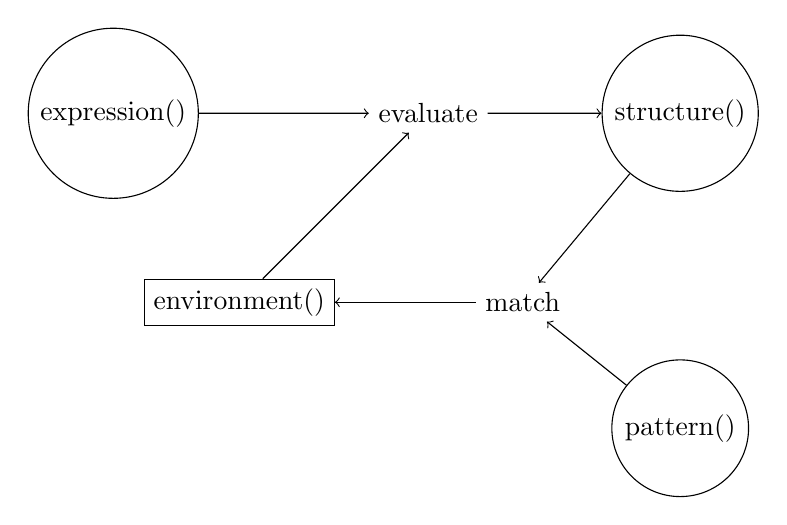
\begin{tikzpicture}[scale=0.4]

 \path (18,12) node[circle, draw]  (str) {structure()};

 \path (18,2) node[circle, draw]  (pat) {pattern()} ;

 \path (13,6) node (match) {match};

 \path (4,6) node[draw]  (env) {environment()};

 \draw [->] (str) to [] (match);
 \draw [->] (pat) to [] (match);
 \draw [->] (match) to [] (env);

 \pause

 \path (0,12) node[circle, draw]  (exp) {expression()};

 \path (10, 12) node (eval) {evaluate}; 
 \draw [->] (exp) to [] (eval);
 \draw [->] (env) to [] (eval);

 \pause

 \draw [->] (eval) to [] (str);


\end{tikzpicture}


\end{frame}

\begin{frame}[fragile]{a sequence}

A sequence consist of a zero or more pattern matching expressions followed by an expression.

\pause\vspace{20pt}

\verb+ X = a, Y = [X|[]], [b|Y]+

\pause\vspace{20pt}
\begin{verbatim}
  [{match, {var, x}, {atm, a}},
   {match, {var, y}, {cons, {var, x}, {atm, []]}},
   {cons, {atm, b}, {varm y}}]
\end{verbatim}

\end{frame}


\begin{frame}[fragile]{a sequence}

\begin{verbatim}
-spec eval_seq([expression()]) -> {ok, structure()} | error.
\end{verbatim}
\pause\vspace{20pt}

\begin{verbatim}
eval_seq([Exp], Env) ->
    eval_expr(Exp, Env);
eval_seq([{match, Ptr, Exp}|Seq], Env) ->
    case eval_expr(Exp, Env) of
      {ok, Str} ->
          case match(Ptr, Str, Env) of
             {ok, Updated} ->
                 eval_seq(Seq, Updated);
             fail ->
                 error
          end;
       error ->
          error 
     end.
\end{verbatim}

\end{frame}

\begin{frame}[fragile]{match}

When matching a pattern with a data structure we will either {\em
fail} or return a substition i.e. an extended environment containing the new
bindings.

\begin{verbatim}
-spec match(pattern(), structure(), environment()) -> 
          {ok, environment()} | fail.
\end{verbatim}

\end{frame}


\begin{frame}[fragile]{match}

\begin{verbatim}
match({atm, Id}, Id, Env) ->    
    {ok, Env};
\end{verbatim}
\pause
\begin{verbatim}
match({var, Id}, Str Env) -> 
    case env:lookup(Id, Env) of
        {Id, Str} ->
            {ok, Env};
        {Id, _} ->
            fail;
        false ->
            {ok, env:add(Id, Str, Env)}
    end;
\end{verbatim}
\end{frame}

\begin{frame}[fragile]{match}

\begin{verbatim}
match({cons, Hp, Tp}, [Hs|Ts], Env) -> 
    case match(Hp, Hs, Env) of
        {ok, Upd} ->
            match(Tp, Ts, Upd);
        fail ->
            fail
    end;
\end{verbatim}

\end{frame}

\begin{frame}[fragile]{match}
\begin{verbatim}
match(ignore, _, Env) ->
    {ok, Env};
\end{verbatim}
\pause
\begin{verbatim}
match(_, _, _) -> 
    fail.
\end{verbatim}

\end{frame}


\begin{frame}[fragile]{eval\_exp}

Evaluating an exression given an environment will return a data structure.

\pause\vspace{20pt}

\begin{verbatim}
-spec eval_exp(expression(), environment()) -> 
          structure().
\end{verbatim}

\end{frame}


\begin{frame}[fragile]{evaluate terms}

\begin{verbatim}
eval_expr({atm, A},_) ->
   {ok, A};
\end{verbatim}
\pause
\begin{verbatim}
eval_expr({var, V}, Env) ->
   case env:lookup(V, Env) of
      {V, S} ->
           {ok, S};
      false ->
           error
    end.
\end{verbatim}
\pause
\begin{verbatim}
eval_expr({cons, Head, Tail}, Env) ->
    case eval_expr(Head, Env) of
      {ok, H} ->
         case  eval_expr(Tail, Env) of
            {ok, T} ->
                {ok, [H|T]};
            error ->
                 error
          end;
       error ->
          error
     end.
\end{verbatim}
\pause\vspace{20pt}
\verb+ eval_expr({cons, {var, x}, {atom, []}}, env:bind(x, a))+
\pause\vspace{10pt}
\verb+ {ok, [a]}+
\end{frame}


\begin{frame}[fragile]{case expression}

\begin{verbatim}
  case [a] of
    [] -> false;
    [X|_] ->  >
  end.
\end{verbatim}

{\em \verb+case+ is a reserved symbol}
\pause

\begin{verbatim}
-type case() :: {switch, expression(), [clause()]}.
\end{verbatim}
\pause
\begin{verbatim}
-type clause() :: {clause, expression(), [expression]}.
\end{verbatim}

\pause
\begin{verbatim}
{switch {cons, {atm, a}, {atm, []}}  
   [ {clause, {atm, []}, [{atm, false}]}
     {clause, {cons, {var, x}, ignore} , [{var, x}]}
   ]}
\end{verbatim}

\end{frame}

\begin{frame}[fragile]{case expression}

\begin{verbatim}
eval_expr({switch, Expr, Cls}, Env) ->
    case eval_expr(Expr, Env) of
       {ok, Str} ->
           eval_cls(Str, Cls, Env);
        error ->
           error
    end.
\end{verbatim}

\pause
\begin{verbatim}
eval_cls(Str, [{clause, Ptr, Seq} | Cls], Env) ->
    case match(Ptr, Str, Env) of
        {ok, Upd} ->
            eval_seq(Seq, Upd);
        fail ->
            eval_cls(Str, Cls, Env)
    end.
\end{verbatim}

\end{frame}

\begin{frame}{what is left}

What is left?

\pause\vspace{20pt}
\begin{itemize}
\item a program : a set of named functions
\item function calls :  {\tt foo(a,b)} 
\item lambda expressions : {\tt fun(X) -> [X] end}
\end{itemize}
        
\pause\vspace{20pt}
{\em .. left as an exercise}

\end{frame}

\begin{frame}{summary}

Erlang, as many functional programming languages, has a small core that is
well defined and simple to describe.

\pause\vspace{20pt}
Advantages: 
\pause
\begin{itemize}
\item easier to describe 
\pause
\item easier to extend 
\pause
\item easier to implement 
\pause
\item easier to analyze
\end{itemize}

\end{frame}

\end{document}


